
% This document is for the Group Meeting Agenda.  The Agenda should
% be distributed to each member (and other invitees) and to the TA
% prior to the meeting (hopefully the day before) so that each member
% will have adequate time to prepare for the meeting.  The best way
% to accomplish the distribution of the agenda is to email the LaTeX
% file to all members and TA.
%
%\documentstyle[fullpage]{article}
\documentclass[a4paper,12pt]{article}
\usepackage{fullpage}
\usepackage{cite}
\usepackage{url}
\usepackage{xcolor}
\usepackage{setspace}
\usepackage[version=4]{mhchem}
\usepackage{upgreek}
\usepackage[margin=0.75in]{geometry}
% For figure:
\usepackage{graphicx}
\usepackage{float}
% For table:
\usepackage{makecell}
\makeatletter
% we use \prefix@<level> only if it is defined
\renewcommand{\@seccntformat}[1]{%
  \ifcsname prefix@#1\endcsname
    \csname prefix@#1\endcsname
  \else
    \csname the#1\endcsname\quad
  \fi}
% define \prefix@section
\newcommand\prefix@section{}
\makeatother
\begin{document}

%
% This section gives the general information about the meeting such
% as the title, who it was called by, when and where the meeting
% will take place, what type of meeting it is (planning, design,
% problem-solving, decision-making, etc.), and of course who is
% invited to attend.
%

\pagestyle{fancyplain}
\fancyhf{}
\lhead{ \fancyplain{}{BIOL 4020 – Vertebrate Biodiversity - ``Fishes''}}
%\chead{ \fancyplain{}{}}
\rhead{ \fancyplain{}{Fall 2020}}
%\rfoot{\fancyplain{}{page \thepage\ of \pageref{LastPage}}}
\fancyfoot[RO, LE] {page \thepage\ of \pageref{LastPage}}
\thispagestyle{plain}

\section*{Evolutionary trees to know:}
\begin{figure}[H]
\centering
  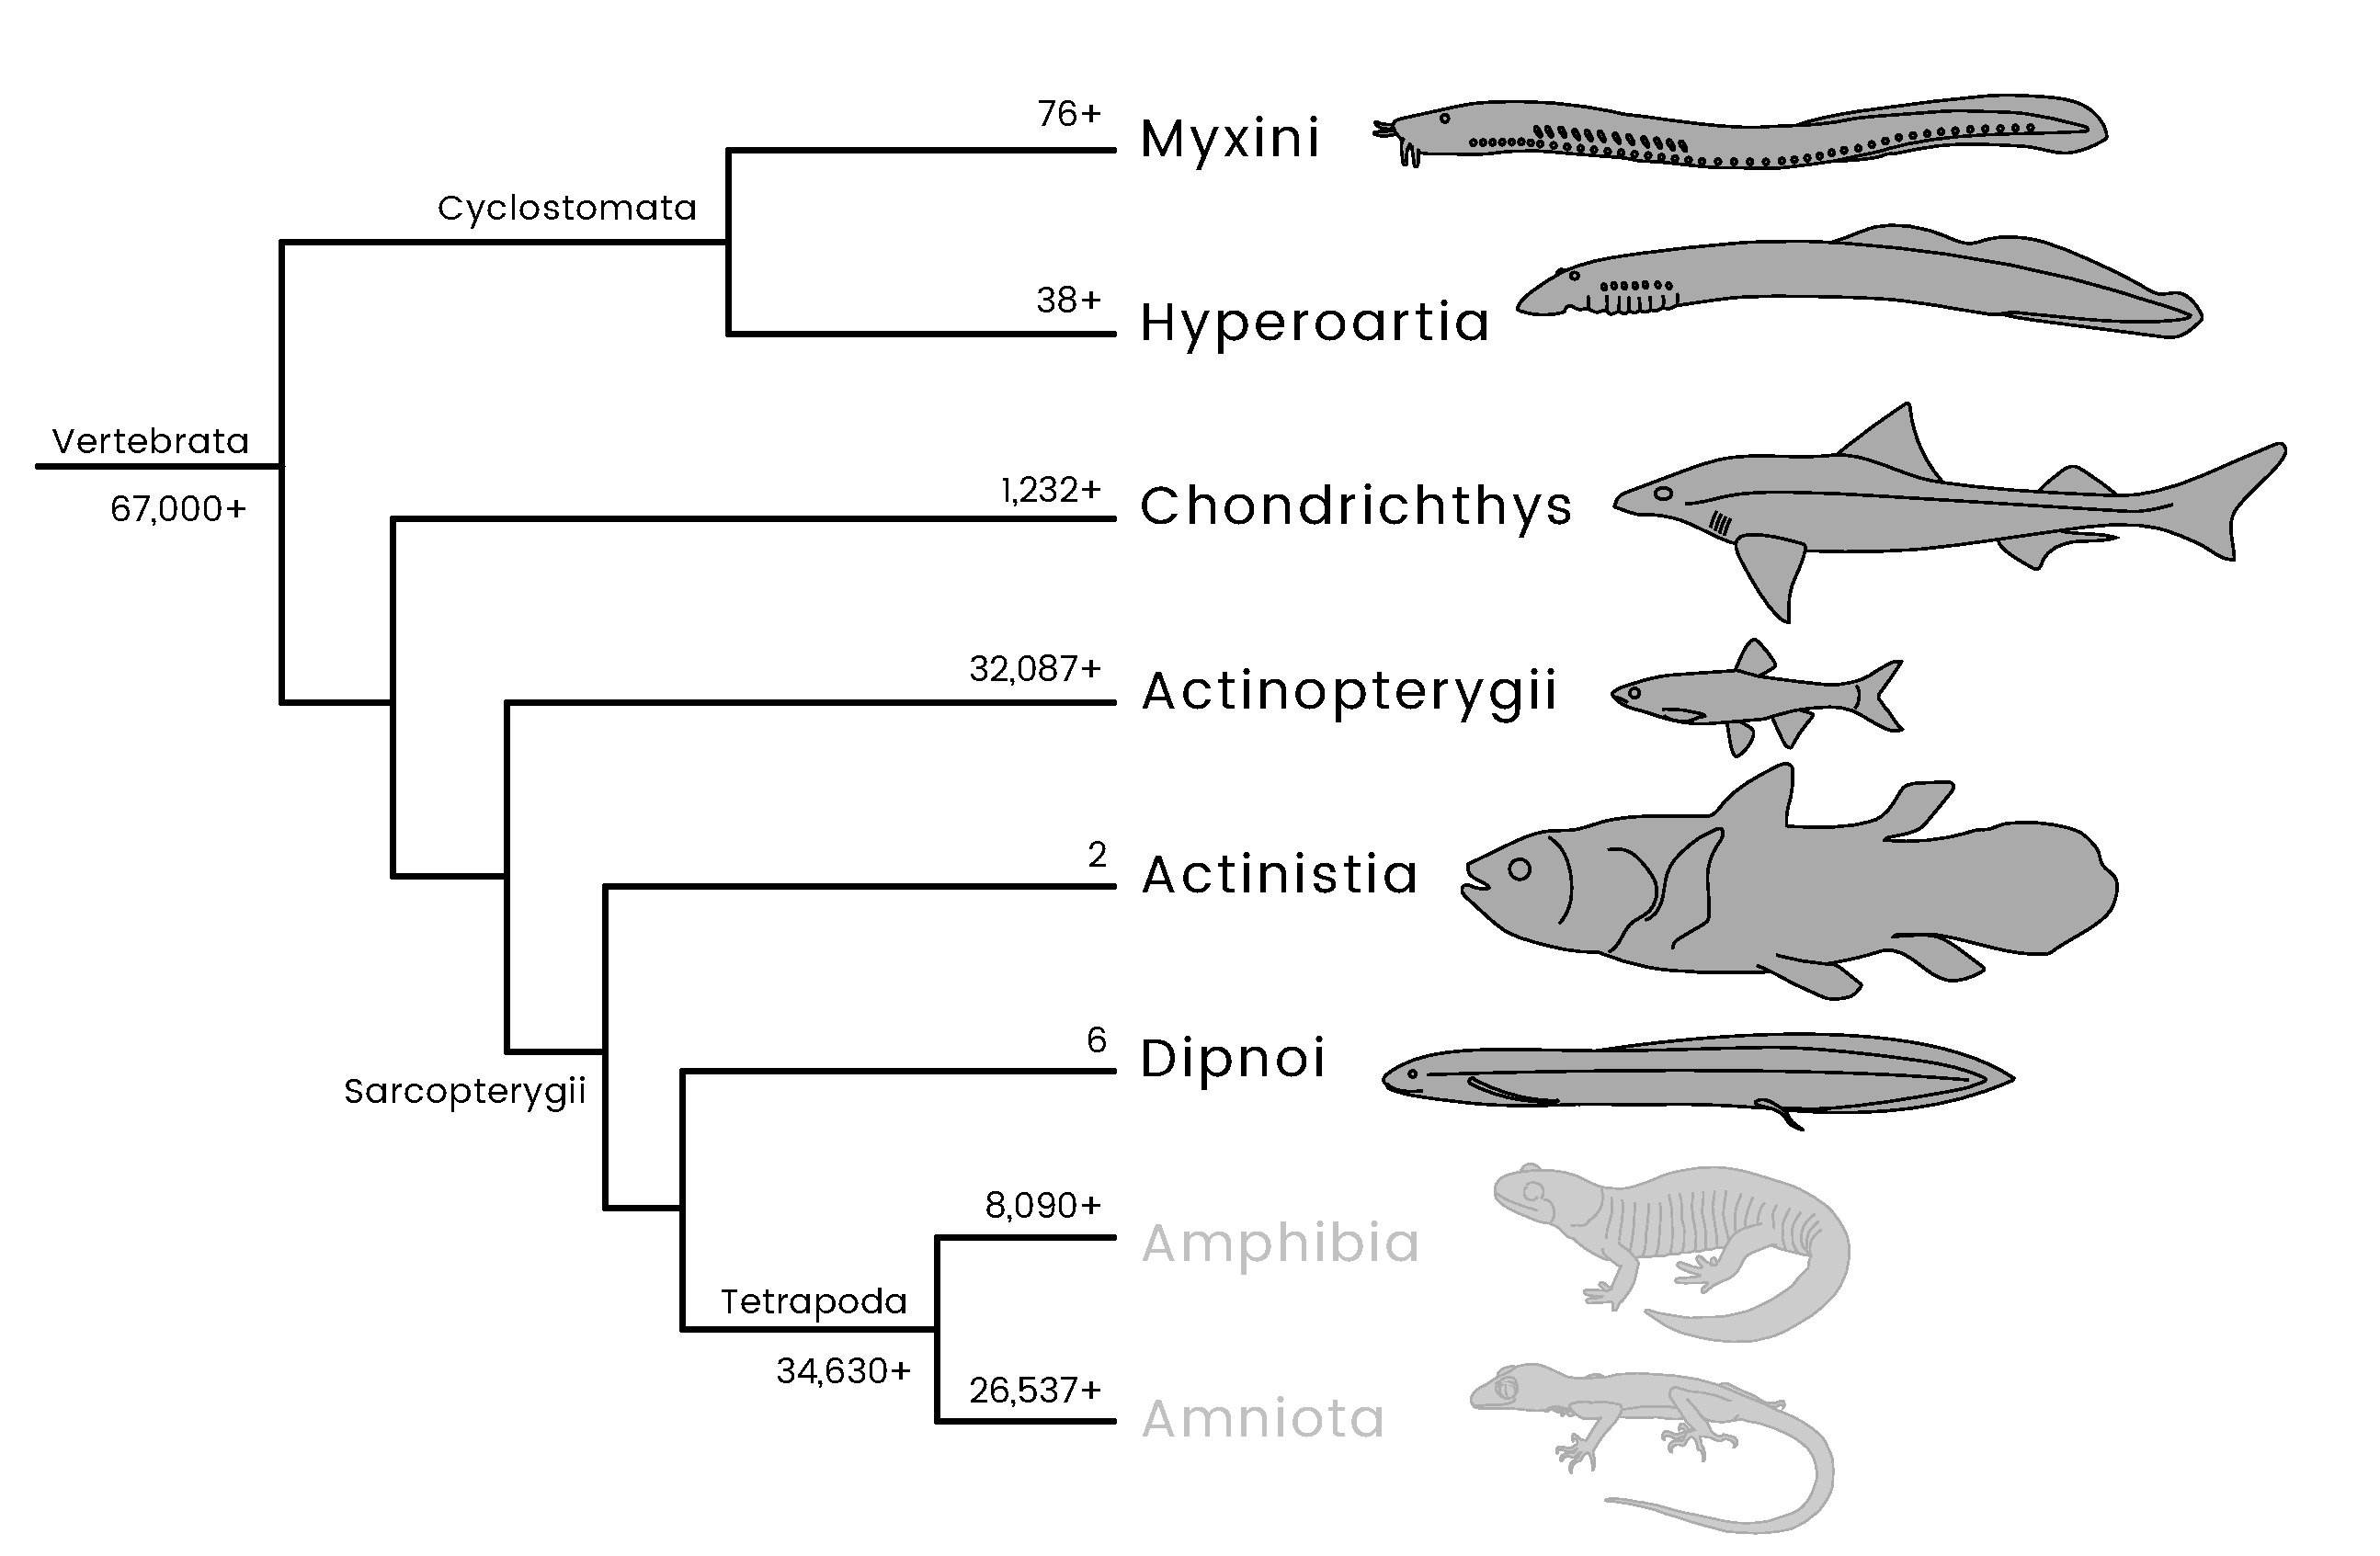
\includegraphics[scale=0.4]{Vertebrata_fishes_tre.pdf}
  \caption{How ``fish'' relate to other vertebrates}
  \label{fig:Fishes}
\end{figure}

%\begin{singlespace}
%\section*{Evolutionary terms to know:}
%\begin{itemize}
%  \large{
%  \item{Monophyly}
%  \item{Clade}
%  \item{Paraphyly}
%  \item{Grade}
%  }
%\end{itemize}
%\end{singlespace}

\begin{figure}[H]
\centering
  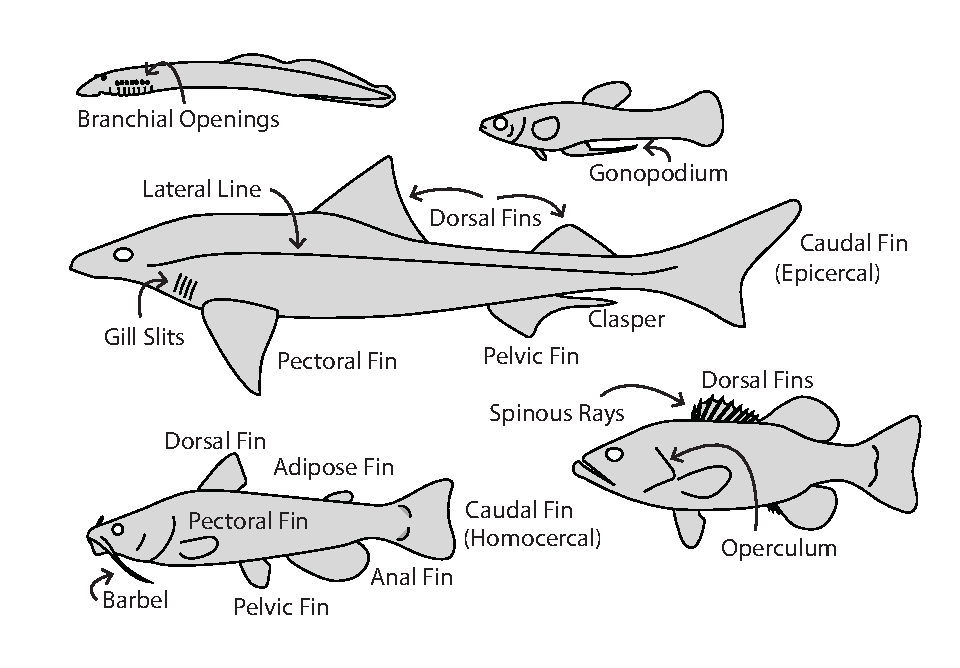
\includegraphics{FishAnatomy.pdf}
  \caption{Fish anatomical terms to know}
  \label{fig:FishAnatomy}
\end{figure}

\section*{Focal taxonomic groups ($\star$ groups you need to be able to photo ID and place in a phylogeny)}
\begin{description}
\item{\underline{{\LARGE{Cyclostomata}}}} (Jawless fish) No vertebral central, no pectoral / pelvic fins with endoskeletal support, gill openings pores rather than slits, elongated body
\begin{itemize}
  \item{\textbf{Myxini} (hagfish) $\star$}\\ 12 pairs of gill openings, mucous glands lateroventraly along the body, Paired of sensing tentacles
  \item{\textbf{Hyperoartia} (lamprey)$\star$}\\ 7 pairs of gill openings, single mediodorsal nostral, funnel-shaped mouth surrounded by oral disk
\end{itemize}
\item\textbf{Gnathostomata} (jawed fish)

\begin{figure}[H]
\centering
  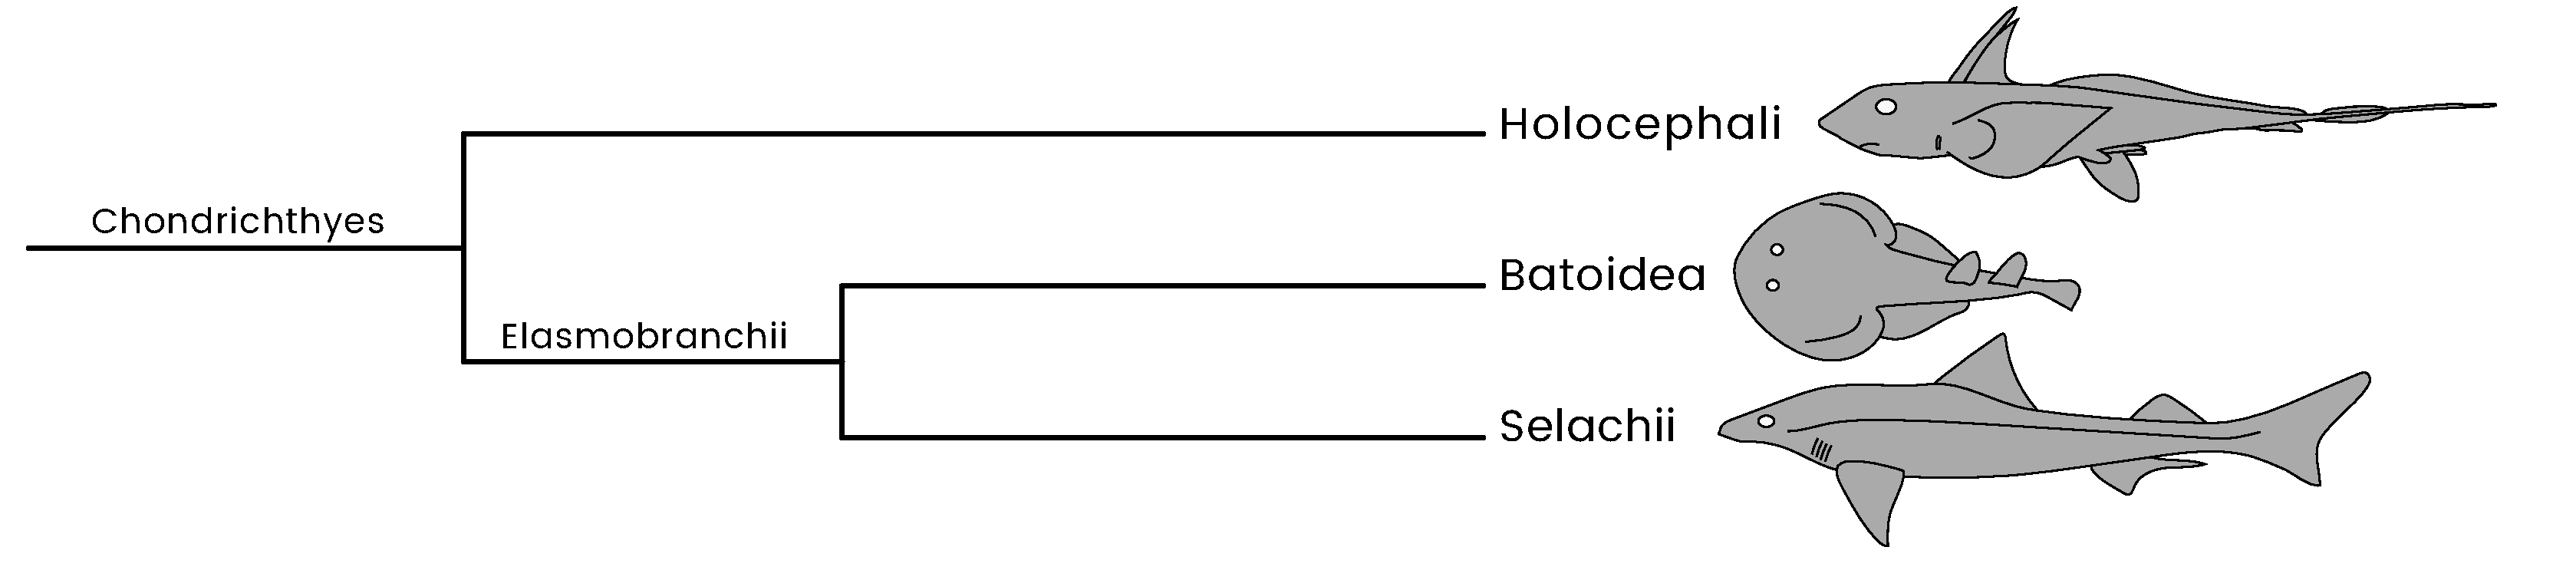
\includegraphics[scale=0.4]{Chondrichthys_tre.pdf}
  \caption{Major groups within Chondrichthys}
  \label{fig:Chondrichthys}
\end{figure}

\item{\underline{{\LARGE{Chondrichthys}}}}
(Cartilagenous fish) Endoskeleton made primarily of cartilage, placoid scales, no swim bladder
\begin{itemize}
  \item{\textbf{Holocephali} (Chimaera)$\star$}\\ Operculum over 4 gill arches, teeth are grinding plates, no cloaca (anal anurogenital openings separate)
  \item{\textbf{Elasmobranchii}} \\ Heterocercal tail, internal fertilization via claspers
  \begin{itemize}
    \item{\textbf{Selachii} (Sharks)$\star$}\\ Heterocercal tail, 5-7 exposed lateral gill slits anterior to pectoral fins
    \item{\textbf{Batoidea} (Skates \& Rays)$\star$} \\ Dorsoventrally flattened body, expanded pectoral fins fused to the head
  \end{itemize}
\end{itemize}


\begin{figure}[H]
\centering
  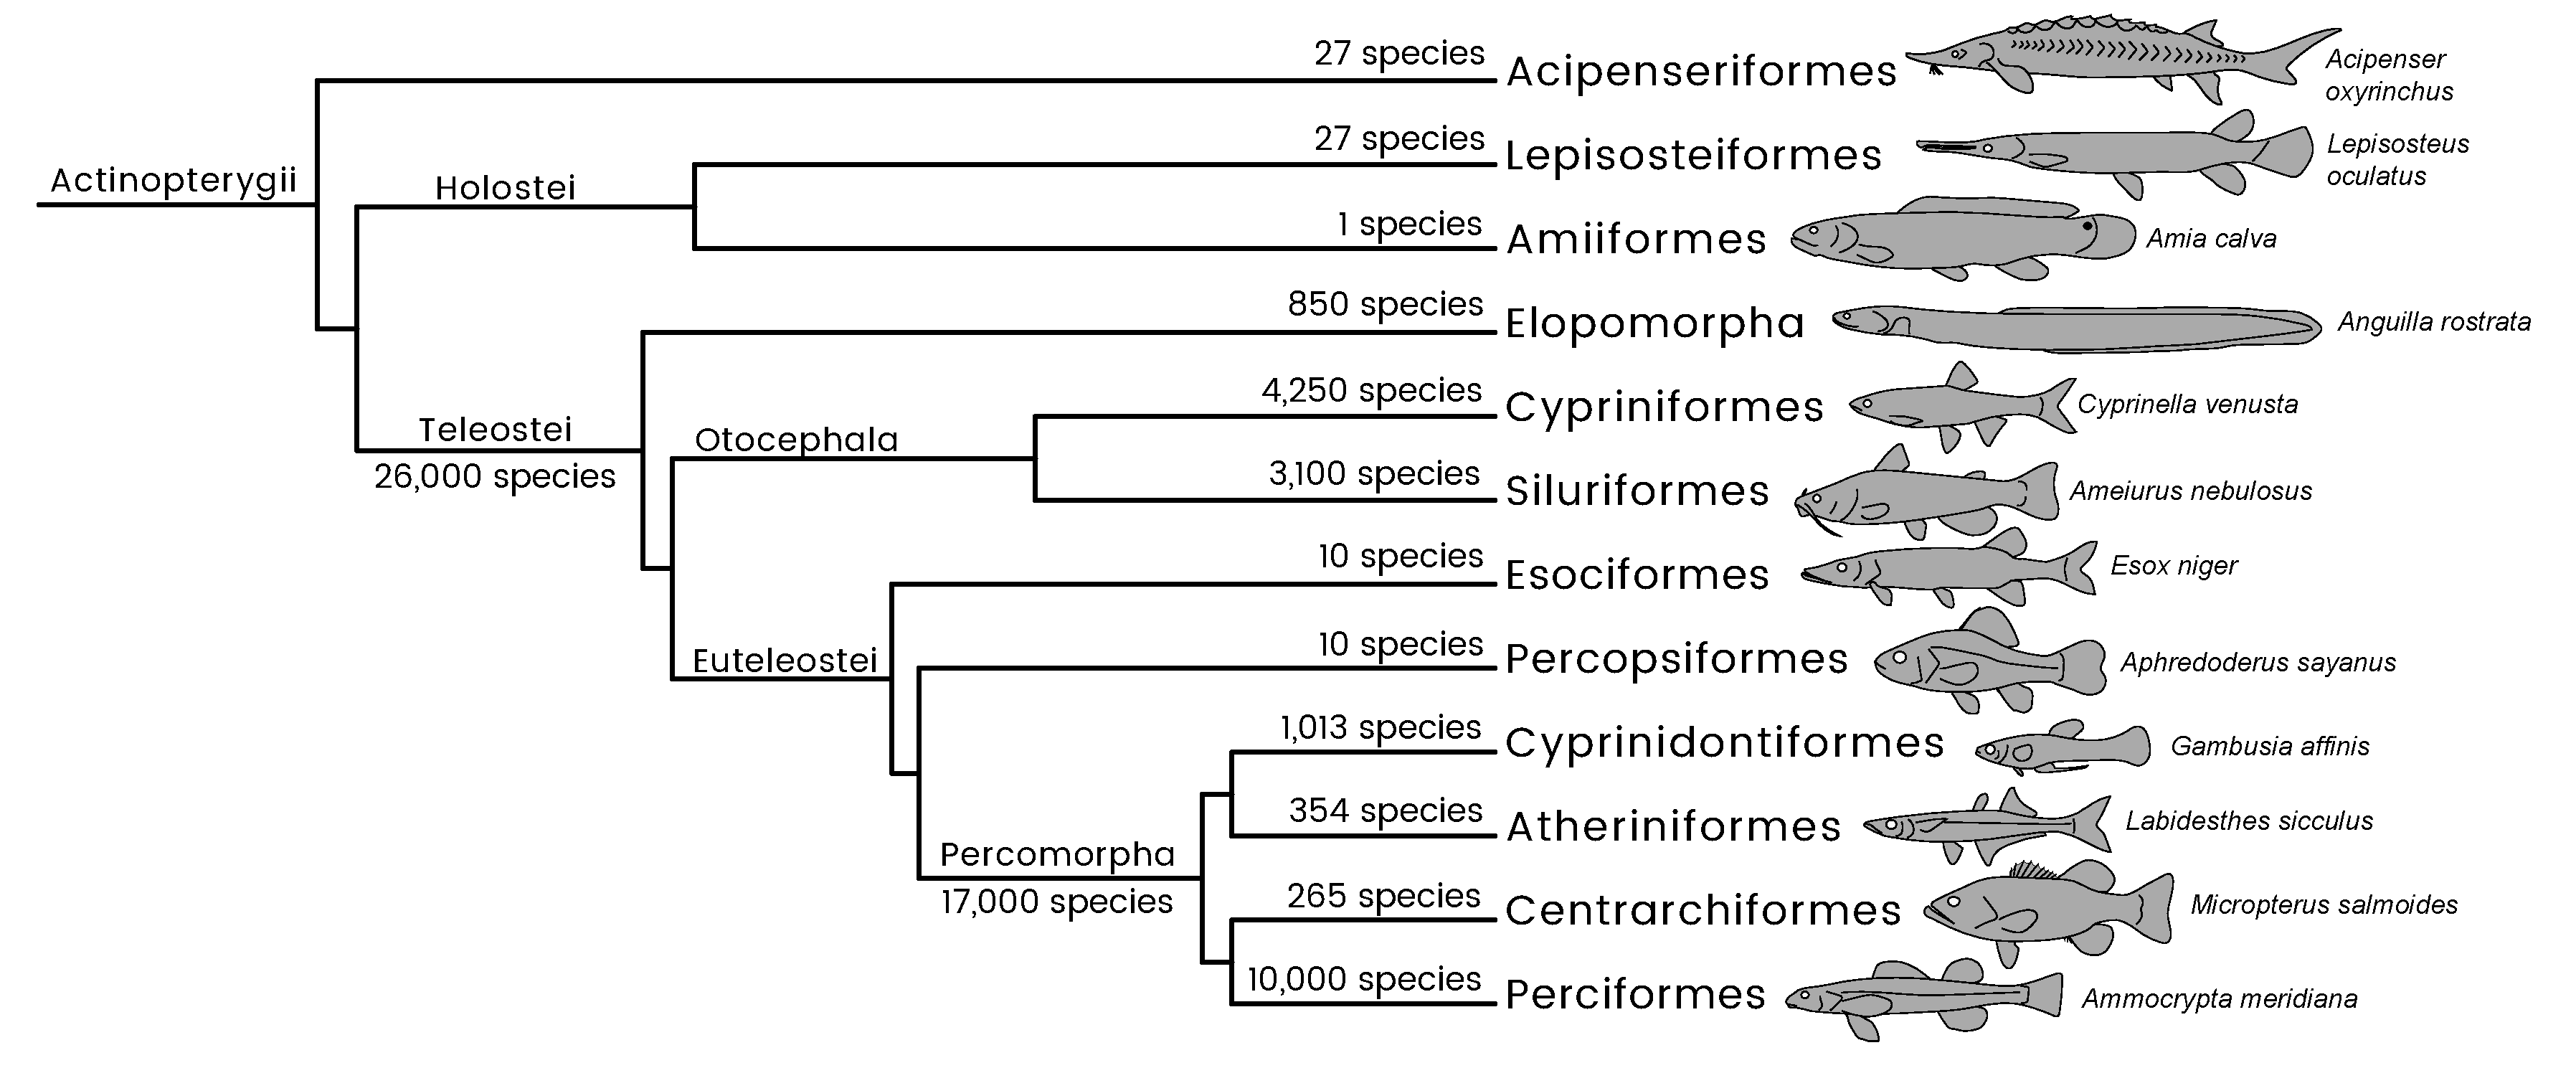
\includegraphics[scale=0.4]{Actinopterygii_tre.pdf}
  \caption{Major groups within Actinopterygii}
  \label{fig:Actinopterygii}
\end{figure}

\item{\underline{{\LARGE{Actinopterygii}}}}
Raylike supports in fins, radial bones of pectoral girdle all attached to the scapulocoracoid complex
\begin{itemize}
  \item{\textbf{Acipenseriformes}} \\ Heterocercal tail, only dermal bones of head and pectoral girdle ossified
  \begin{itemize}
    \item{\textbf{family ACIPENSERIDAE} (sturgeons)} \\ Robust body armed with 5 longitudinal rows of large bony plates, pronounced snout with 4 sensitive barbels, largest freshwater fish
      \item{\textbf{\textit{   Scaphirhynchus platorynchus}} (shovel-nosed sturgeon)$\star$} \\ highly endangered, 4 lobes on lower lip, fringed barbels on front of mouth
    \item{\textbf{family POLYODONTIDAE} (paddlefish)} \\ paddle/spatula-like snout, virtually naked skin, greatly extended operculum
      \item{\textbf{\textit{   Polyodon spathula}} (American paddlefish)$\star$} \\ grows up to 7 ft, filter-feeder
  \end{itemize}
  \item{\textbf{Lepisosteiformes} (gars)$\star$} \\ elongate jaws with teeth, elongate body with dorsal and anal fins located caudally, abbreviated heterocercal tail, swim bladder can be used for respiration
  \begin{itemize}
    \item{\textbf{\textit{   Lepisosteus oculatus}} (spotted gar)} \\ olive brown to black, spots on body, head, and fins
  \end{itemize}
  \item{\textbf{Amiiformes} (bowfin)} \\ swim bladder can be used for respiration, round snout
  \begin{itemize}
    \item{\textbf{\textit{   Amia calva}} (bowfin)$\star$} \\ body nearly cylindrical, long dorsal fin, abbreviated heterocercal tail, gular plate
  \end{itemize}
  \item{\textbf{Elopomorpha}} \\ Leptocephalus larvae
  \begin{itemize}
    \item{\textbf{Anguilliformes} (eels)} \\ body elongate, lack pelvic fins, pelvic girdle is often absent and when present is remote from skull
    \item{\textbf{\textit{   Anguilla rostrata}} (American eel)$\star$} \\ long anal and dorsal fins
  \end{itemize}
  \item{\textbf{Cypriniformes}$\star$} \\ Kinethmoid bone for jaw protrusion
  \begin{itemize}
    \item{\textbf{family CATOSTOMIDAE} (suckers)} \\ Pelvic fins abdominal, 1 dorsal fin, dorsal fin rays 10 or more, large mouth suckers ventral
    \item{\textbf{\textit{   Carpiodes velifer}} (highfin carpsucker)$\star$} \\ Long sickle-shaped dorsal fin, projection on lower lip
    \item{\textbf{\textit{   Hypentelium etowanum}} (Alabama hogsucker)} \\ Cylindrical body, very pronounced ventral sucker, top of head between eyes flat or concave
    \item{\textbf{family CYPRINIDAE} (minnows and carp)} \\ no teeth on jaws, modified teeth on gill arches, fin rays soft and flexible, pelvic fins abdominal
    \item{\textbf{\textit{   Cyprinella venusta}} (black-tail shiner)$\star$} \\ large black spot at base of caudal fin
    \item{\textbf{\textit{   Pimephales vigilax}} (bullhead minnow)} \\ blunt snout, leading ray stout and detached from first principle ray, light tail spot
    \item{\textbf{\textit{   Notropis ammophilus}} (orangefin shiner)} \\ 8 dorsal rays, prominant orange fins
  \end{itemize}
  \item{\textbf{Siluriformes} (catfish)$\star$} \\ Single spinous ray at beginning of dorsal and pectoral fins, adipose fin, pectoral girdle modified to form locking mechanism for pectoral fin spine
  \begin{itemize}
    \item{\textbf{\textit{   Ictalurus punctatus}} (channel catfish)} \\ caudal fin forked, 9 pelvic rays, deeply forked tail
    \item{\textbf{\textit{   Ameiurus nebulosus}} (brown bullhead)$\star$} \\ 8 pelvic rays, caudal fin not deeply forked, white or yellow chin barbels
  \end{itemize}
  \item{\textbf{Esociformes}} \\ Elongate body, tootless maxilla, posterior dorsal and anal fins
  \begin{itemize}
    \item{\textbf{\textit{   Esox niger}} (chain pickerel)$\star$} \\ duckbill-like snout, snout longer than postorbital length of head, abdominal pectoral fins
  \end{itemize}
  \item{\textbf{Percopsiformes}} \\ ctenoid scales, spines on medial fins reduced or lost
  \begin{itemize}
    \item{\textbf{\textit{   Aphredoderus sayanus}$\star$} (pirate perch)} \\ anus anterior between pectoral fins in adults (not in juveniles)
  \end{itemize} 
  \item{\textbf{Cyprinidontiformes}$\star$} \\ unlobed caudal fin, low-set pectoral fins
  \begin{itemize}
    \item{\textbf{family POECILIIDAE} (live-bearers)} \\ small fins, caudal fin rounded, mouth small and directed upward, males have anal fin displaced forward with gonopodium formed from 3 anal rays, elaborate reproductive strategy
    \item{\textbf{\textit{   Gambusia affinis}} (western mosquito fish)$\star$} \\ 6 dorsal fin rays
    \item{\textbf{family FUNDULIDAE} (killifish)} \\ elongate body somewhat laterally compressed with head dorsoventrally flattened, mouth small and turned upward, lower jaw extends beyond upper
    \item{\textbf{\textit{   Fundulus olivaceus}} (black-spotted topminnow)$\star$} \\ Dorsal fin origin posterior from anal fin origin, prominant black stripe with dorsal spotting
  \end{itemize}
  \item{\textbf{Atheriniformes} (silversides)} \\ 2 dorsal fins well separated (first with weak spines), anal fin longer than second dorsal fin, elongate and slightly compressed body
  \begin{itemize}
    \item{\textbf{\textit{   Labidesthes sticculus}} (brook sliverside)$\star$} \\ origin of first dorsal fin near origin of anal fin
  \end{itemize}
  \item{\textbf{Centrarchiformes}$\star$} \\ 2 dorsal fins, 3 or more spines on anal tail, siny dorsal fin confluent with soft dorsal fin
  \begin{itemize}
    \item{\textbf{\textit{   Lepomis cyanellus}} (green sunfish)$\star$} \\ maxilla reaches beneath eye, pectoral fin short and rounded
    \item{\textbf{\textit{   Micropterus salmoides}} (largemouth bass)$\star$} \\ large mouth with lower jaw projecting, smaller spiny dorsal fin separated by notch from the second dorsal fin
  \end{itemize}
  \item{\textbf{Perciformes}$\star$} \\ spines in dorsal and anal fins
  \begin{itemize}
    \item{\textbf{family COTTIDAE} (sculpins)} \\ skin mostly naked, high eyes directed upward, body robust with large head
    \item{\textbf{\textit{   Cottus carolinae}} (banded sculpin)} \\ mottled brown with dark vertical banding, broad head, body narrows caudally
    \item{\textbf{family PERCIDAE} (perches and darters)} \\ two dorsal fins, dorsal fins separated bya  space, 2 anal spines
    \item{\textbf{\textit{   Ammocrypta meridiana}} (southern darter)$\star$} \\ elongate body, blunt snout, caudal fin truncate
  \end{itemize}
\end{itemize}

\item{\underline{{\LARGE{Sarcopterygii}}}}
Radial bones of pectoral girdle not all attached to the scapulocoracoid complex
\begin{itemize}
  \item{\textbf{Actinistia} (lobe-finned fish)$\star$} \\ skull divided anteriorly and posteriorly, widely distributed 400 million years ago
  \item{\textbf{Dipnoi} (lung fish)$\star$} \\ elongated and laterally compressed body, respire by gills and lungs
  \item{\textbf{You!} (Along with all other tetrapods)}
\end{itemize}
\end{description}

\end{document}
